\chapter{Introduction}

\section{First section}

\lipsum[3-4]

\begin{figure}[h]
	\centering
	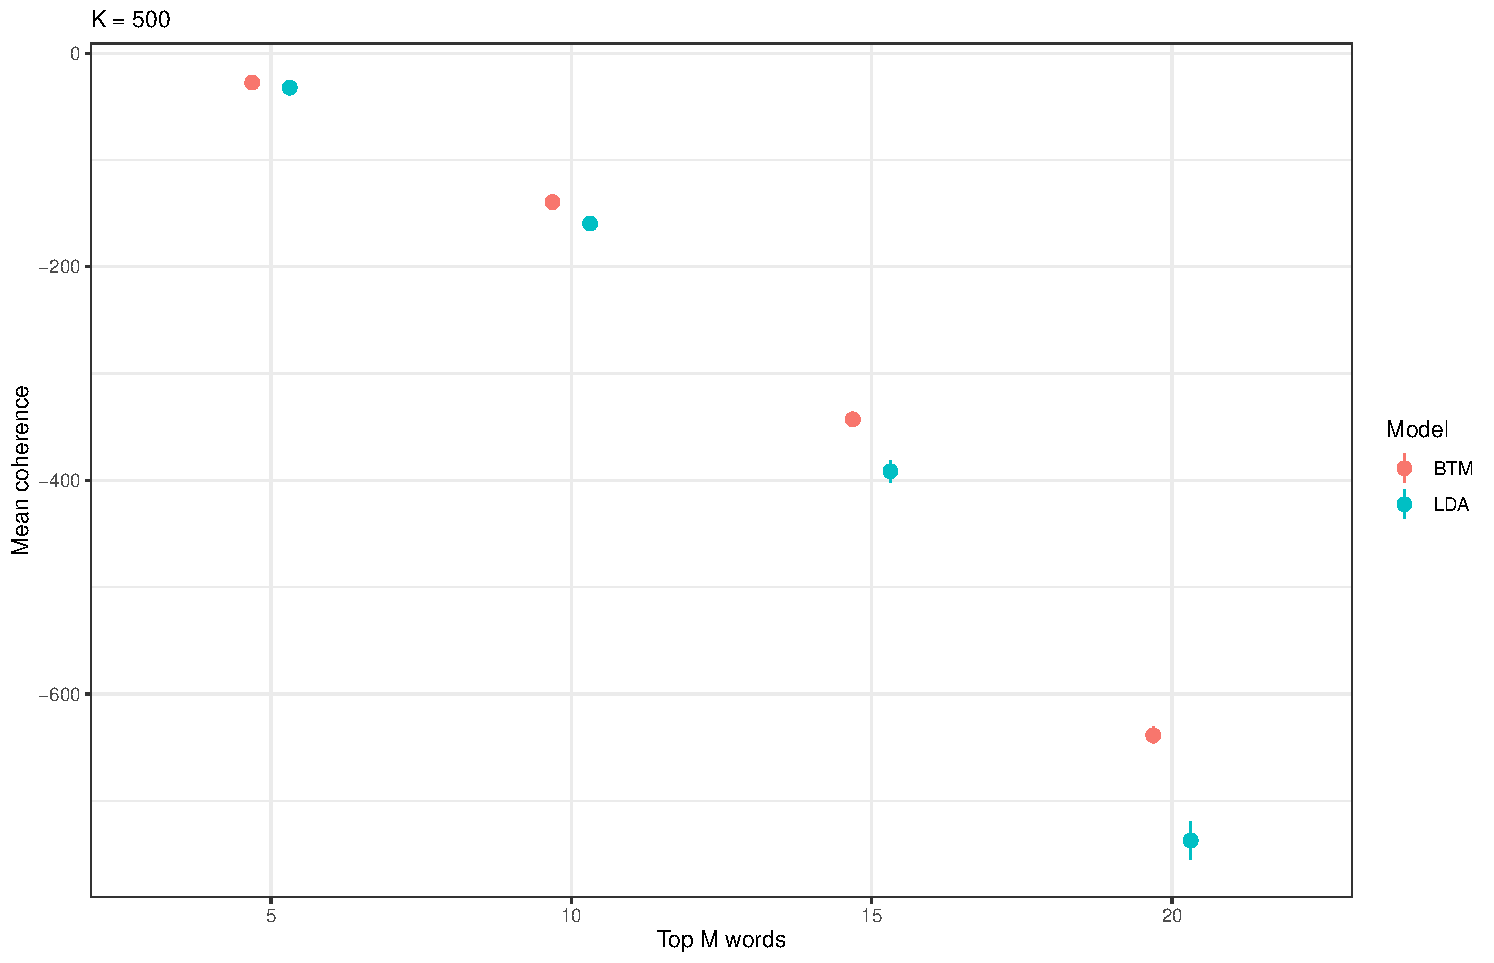
\includegraphics[width=\linewidth]{coherence_k500}
	\caption{\label{fig:coherence}This caption explains the above plot.}
\end{figure}

\lipsum[5]
Looking at the figure above (\autoref{fig:coherence}), I don't remember what I was going to say.


\section{Second section}

\subsection{First subsection}

\lipsum[6-7]

\subsection{Second subsection}

\lipsum[11-12]

\section{Third section}

Everything I do is in R 4.0\supercite{R-4.0.0}. \ttt{purrr}\supercite{purrr} is a great package. I also used a
bunch of other packages\supercite{qs,dplyr,ggplot2}.

\printbibliography[heading=subbibintoc,title={From reading list},keyword={reading}]

\printbibliography[heading=subbibintoc,title={Supplementary readings},notkeyword={reading}]
